\appendix
% Delete the text and write Appendix here (not required, can be omitted):
% Comment out ' \appendix
% Delete the text and write Appendix here (not required, can be omitted):
% Comment out ' \appendix
% Delete the text and write Appendix here (not required, can be omitted):
% Comment out ' \appendix
% Delete the text and write Appendix here (not required, can be omitted):
% Comment out ' \input{Text/Appendix} ' to remove this section.
%------------------------------------

\section{Notes on interpolation}

In a 2d space interpolations car be relatively simple, let's consider the following :

\begin{align} 
    (x,y) \in (R,R)
\end{align}

Let us suppose there is some kind of function linking the two, we hence have :

\begin{align} 
    f(x) = y
\end{align}

Should we consider two points of the function $(x_0,y_0)$ and $(x_1,y_1)$ and seek to find the value of a given unknown third point $(x_a,y_a)$ then one would instinctively do a linear interpolation as follows :

\begin{align} 
    \frac{x_1-x_0}{y_1-y_0} (x_a-x_0) + y_0 = y_a
    \label{eq:interp1d}
\end{align}

Should we desire to interpolate at a higher order, we can use the Lagrange set of polynomes as follows:

\begin{align} 
    y(x) = \sum_{j=0}^{k} y_j c_j(x)
        c_j(x) = \ell_j(x,x_0,x_1,\ldots,x_k) = \nonumber \\
        \prod_{\begin{smallmatrix}0\le m\le k\\ m\neq j\end{smallmatrix}} \frac{x-x_m}{x_j-x_m} = \nonumber \\
        \frac{(x-x_0)}{(x_j-x_0)} \cdots \frac{(x-x_{j-1})}{(x_j-x_{j-1})} \frac{(x-x_{j+1})}{(x_j-x_{j+1})} \cdots \frac{(x-x_k)}{(x_j-x_k)}
\end{align}

For a polynome of order $k$ we require $k+1$ node points, this is an important point to keep in mind when constructing a grid to subsequently interpolate. Interpolation residuals will not be detailed here. As all that is explicated here can be found in any math book, the more curious reader can quite easily find further details.

Another way of of seeing \cref{eq:interp1d} is as evaluating the barycenter along a line. where the term $x_a-x_0$ represents the displacement from $x_0$ to $x$. Generalised, it is possible to write the higher order polynomial approximation in terms of the displacement from a given point.

\begin{align} 
    L(x) = \ell(x) \sum_{j=0}^k \frac{w_j}{x-x_j}y_j
\end{align}

In practice this means that we consider a set of values $f(x_j)=y_j$ close to the desired point and interpolate the point by weighting the $f(x_j)$ values by the distance $x-x_j$ to that given point.

That which is given here is valid in a two dimensional space but for parts of the work, it is required to interpolate in higher dimension. To quote "Méthode numériques appliquées" by Jean-Philippe Grivet \parencite{Methodes_numerique_appliques} : "The algorithms described above can be generalized in a more or less laborious way to two or more dimensions." This has been one of the challenges to overcome in this work. Indeed for perfectly regular grids, it is possible to derive semi-analytical equations using methods such as bi-cubic interpolations, however here our grids will, through iterative steps, no longer be regular. We propose to overcome this problem to use a barycentric interpolation using a Delauney triangulation. In terms of the barycentric interpolation the method is the same as the logic presented above. We weight the distance between nodes by the distance to the desired point and that for a group of points that surround our point of interest. However the surrounding of a point in higher dimension is a non negligible task. A Delaunay triangulation in a two dimensional space is a triangulation for which no point of the grid is in the circumcircle of another triangle, where a triangle is defined by three points of the grid. If one draws this condition out one will notice that this splits a space into triangles with no points inside those triangles. For a higher dimensional space, the circumcircle becomes a circum-hypersphere. The mathematical details will be left to the most curious readers.\par

In practice, the methods presented were not coded but imported from the python Scipy library. However it is essential when using interpolations to know what is being done. Interpolations if used incorrectly can lead to erroneous results which can appear correct. For this reason we do not explicit extrapolations as any desired data points outside of the grid are deemed only accessible if the grid is extended by running the underlying models. This poses a new challenge, how to correctly extend the grid in order to subsequently perform interpolations. If computational time is plenteous than a random grid search can be completed, otherwise an extrapolation can be carried out with the objective of running the underlying models at the extrapolation point. This is yet to be correctly done.

\section{Notes on degeneracy}

\Cref{fig:Degen} gives an example of partial ternary degeneracy plot generated with Exoris where we see how the radius for a planet at a given mass varies depending on its mass fraction composition. Where the color is the same, we have a degeneracy. We see that it is possible to have the same radius for various mass fractions of hydrogen, helium and core. This plot explicates the need to link interior models with atmosphere models. Indeed the hydrogen and helium mass fractions here are ultimately fixed by the atmosphere model. The core is therefore left as a free parameter, however if the radius of a planet is known it is possible to remove all degeneracy presented here. The more critical reader could think that fundamentally this is just pushing the problem up into the atmosphere, this is true, however as photons escape from radiative zones in the atmosphere, it is theoretically possible with a perfect observation to resolve this internal structure as presented here. However internal structures can be more complex than this diagram indicates. The core can have rock and ice composition, with distinct fractions of both. We can also imagine for Neptune like planets layers of water/ice in the envelope, in which case the degeneracy plot becomes more complicated and further work is required in order to understand what remains degenerate after model linkage.

\begin{figure}
    \centering
    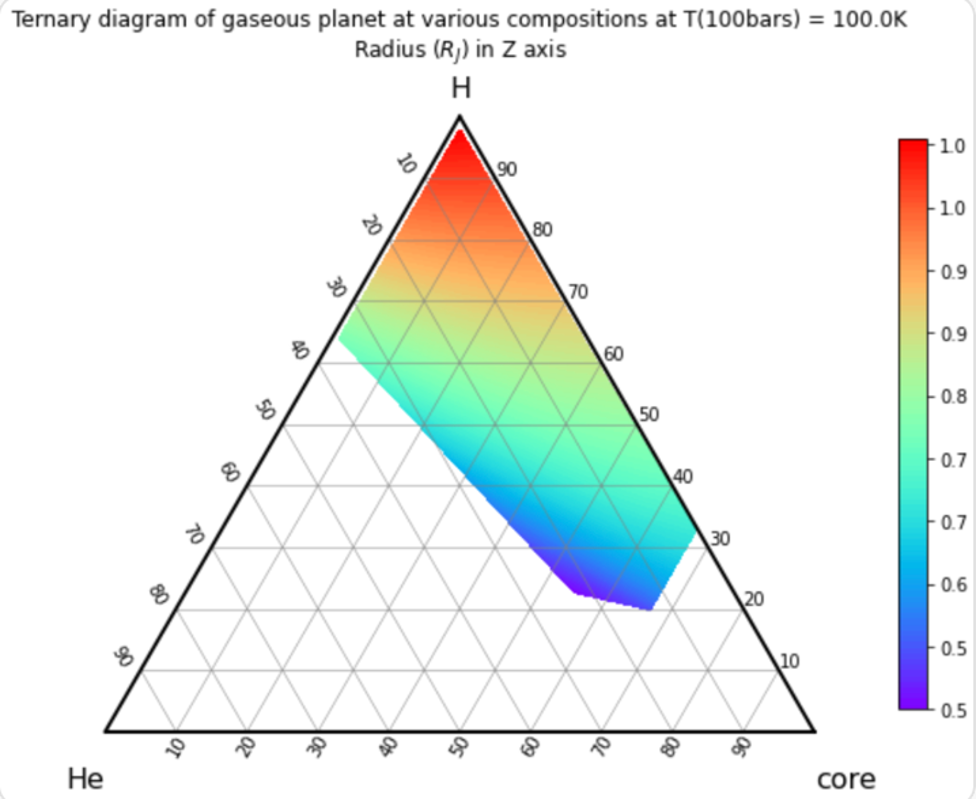
\includegraphics[width=0.48\textwidth]{Images/degeneracies.png}
    \caption{Degeneracy plot (ternary plot), representing radius ($R_J$) at various, hydrogen, helium and core mass fractions}
    \label{fig:Degen}
\end{figure}

\section{Notes on exorem model selection}

As stated in the model description, exorem can in certain conditions struggle to converge. This happens generally in zones of the grid where the irradiation temperature is low and internal temperature high. Exorem can not balance the two stream flux model and balance the temperature at the bottom and top of the atmosphere. To deal with this, we help Exorem converge either by relying on T. Guillot (2010) \parencite{guillot_radiative_2010} non grey analytical model to provide initial pressure temperature profiles to guide exorem, these do not take into account irradiation. We can also re-inject profiles from the grid into Exorem, to accomplish this we find the closest profile to the given input parameters. However often this does not suffice and we still have non-converged profiles. It would be taking a risk to leave these profiles in the grid especially taking into account that for the moment we do not use any smoothing in the interpolation methods considered above. As such we chose to remove these profiles. Through trial and error it was shown that a systematic code to identify bad profiles was inefficient. As such a simple tree based model was used to identify such profiles. To do this a LGBM classifier was trained. LGBM classifiers are gradient boosted tree based learning algorithms that have low memory usage and are more efficient than most other classifiers such as random forests. They use leaf wise tree growth which increases efficiency. The disadvantage of such classifiers are that they are very sensitive to over-fitting and require relatively large data-sets. The model was trained using the top atmosphere flux ratio, bottom atmosphere flux ratio, effective temperature ratio, internal temperature and irradiation temperature. The more data science orientated reader might be concerned when seeing that dimensional data was used as a feature. We allowed ourselves to do this as the internal temperature and irradiation temperature are bounded by the grid limits, rigorously one should divide these values by their maximum value on the grid. The results obtained were an accurate categorisation of 98\% of profiles, with an equal split percentage wise between false positives and false negatives. 

\section{Notes on entropy of mixes}

As shown in \parencite{chabrier_new_2019}, the expression for a given extensive quantity $W$ at a given $(T,P)$ for a mixture is given by :

\begin{align} 
    W(T,P) = \sum_{i} X_{i} W_{i}(T,P)
    \label{eq:extensive_qty}
\end{align}

With :

\begin{align} 
    X_{i} = \frac{M_i}{\sum_{i}M_{i}}
    \label{eq:mass_fraction}
\end{align}

Subsequently we can express the entropy of a mix of $He/H/H_2O$ as follows :

\begin{align} 
    S = \sum_{i} X_{i} S_{i}(T,P) + S_{mix}(T,P)
    \label{eq:entropy_mix1}
\end{align}

\begin{align} 
    S = X_{H} S_{H}(T,P) + X_{He} S_{He}(T,P) \nonumber \\ 
    + X_{H_2O} S_{H_2O}(T,P) + S_{mix}(T,P)
    \label{eq:entropy_mix2}
\end{align}

With here $S_{mix}(T,P)$ the ideal mixing term that we will better define subsequently. But we shall consider equal to zero.

We need to substitute the expressions for the mass fractions.  ' to remove this section.
%------------------------------------

\section{Notes on interpolation}

In a 2d space interpolations car be relatively simple, let's consider the following :

\begin{align} 
    (x,y) \in (R,R)
\end{align}

Let us suppose there is some kind of function linking the two, we hence have :

\begin{align} 
    f(x) = y
\end{align}

Should we consider two points of the function $(x_0,y_0)$ and $(x_1,y_1)$ and seek to find the value of a given unknown third point $(x_a,y_a)$ then one would instinctively do a linear interpolation as follows :

\begin{align} 
    \frac{x_1-x_0}{y_1-y_0} (x_a-x_0) + y_0 = y_a
    \label{eq:interp1d}
\end{align}

Should we desire to interpolate at a higher order, we can use the Lagrange set of polynomes as follows:

\begin{align} 
    y(x) = \sum_{j=0}^{k} y_j c_j(x)
        c_j(x) = \ell_j(x,x_0,x_1,\ldots,x_k) = \nonumber \\
        \prod_{\begin{smallmatrix}0\le m\le k\\ m\neq j\end{smallmatrix}} \frac{x-x_m}{x_j-x_m} = \nonumber \\
        \frac{(x-x_0)}{(x_j-x_0)} \cdots \frac{(x-x_{j-1})}{(x_j-x_{j-1})} \frac{(x-x_{j+1})}{(x_j-x_{j+1})} \cdots \frac{(x-x_k)}{(x_j-x_k)}
\end{align}

For a polynome of order $k$ we require $k+1$ node points, this is an important point to keep in mind when constructing a grid to subsequently interpolate. Interpolation residuals will not be detailed here. As all that is explicated here can be found in any math book, the more curious reader can quite easily find further details.

Another way of of seeing \cref{eq:interp1d} is as evaluating the barycenter along a line. where the term $x_a-x_0$ represents the displacement from $x_0$ to $x$. Generalised, it is possible to write the higher order polynomial approximation in terms of the displacement from a given point.

\begin{align} 
    L(x) = \ell(x) \sum_{j=0}^k \frac{w_j}{x-x_j}y_j
\end{align}

In practice this means that we consider a set of values $f(x_j)=y_j$ close to the desired point and interpolate the point by weighting the $f(x_j)$ values by the distance $x-x_j$ to that given point.

That which is given here is valid in a two dimensional space but for parts of the work, it is required to interpolate in higher dimension. To quote "Méthode numériques appliquées" by Jean-Philippe Grivet \parencite{Methodes_numerique_appliques} : "The algorithms described above can be generalized in a more or less laborious way to two or more dimensions." This has been one of the challenges to overcome in this work. Indeed for perfectly regular grids, it is possible to derive semi-analytical equations using methods such as bi-cubic interpolations, however here our grids will, through iterative steps, no longer be regular. We propose to overcome this problem to use a barycentric interpolation using a Delauney triangulation. In terms of the barycentric interpolation the method is the same as the logic presented above. We weight the distance between nodes by the distance to the desired point and that for a group of points that surround our point of interest. However the surrounding of a point in higher dimension is a non negligible task. A Delaunay triangulation in a two dimensional space is a triangulation for which no point of the grid is in the circumcircle of another triangle, where a triangle is defined by three points of the grid. If one draws this condition out one will notice that this splits a space into triangles with no points inside those triangles. For a higher dimensional space, the circumcircle becomes a circum-hypersphere. The mathematical details will be left to the most curious readers.\par

In practice, the methods presented were not coded but imported from the python Scipy library. However it is essential when using interpolations to know what is being done. Interpolations if used incorrectly can lead to erroneous results which can appear correct. For this reason we do not explicit extrapolations as any desired data points outside of the grid are deemed only accessible if the grid is extended by running the underlying models. This poses a new challenge, how to correctly extend the grid in order to subsequently perform interpolations. If computational time is plenteous than a random grid search can be completed, otherwise an extrapolation can be carried out with the objective of running the underlying models at the extrapolation point. This is yet to be correctly done.

\section{Notes on degeneracy}

\Cref{fig:Degen} gives an example of partial ternary degeneracy plot generated with Exoris where we see how the radius for a planet at a given mass varies depending on its mass fraction composition. Where the color is the same, we have a degeneracy. We see that it is possible to have the same radius for various mass fractions of hydrogen, helium and core. This plot explicates the need to link interior models with atmosphere models. Indeed the hydrogen and helium mass fractions here are ultimately fixed by the atmosphere model. The core is therefore left as a free parameter, however if the radius of a planet is known it is possible to remove all degeneracy presented here. The more critical reader could think that fundamentally this is just pushing the problem up into the atmosphere, this is true, however as photons escape from radiative zones in the atmosphere, it is theoretically possible with a perfect observation to resolve this internal structure as presented here. However internal structures can be more complex than this diagram indicates. The core can have rock and ice composition, with distinct fractions of both. We can also imagine for Neptune like planets layers of water/ice in the envelope, in which case the degeneracy plot becomes more complicated and further work is required in order to understand what remains degenerate after model linkage.

\begin{figure}
    \centering
    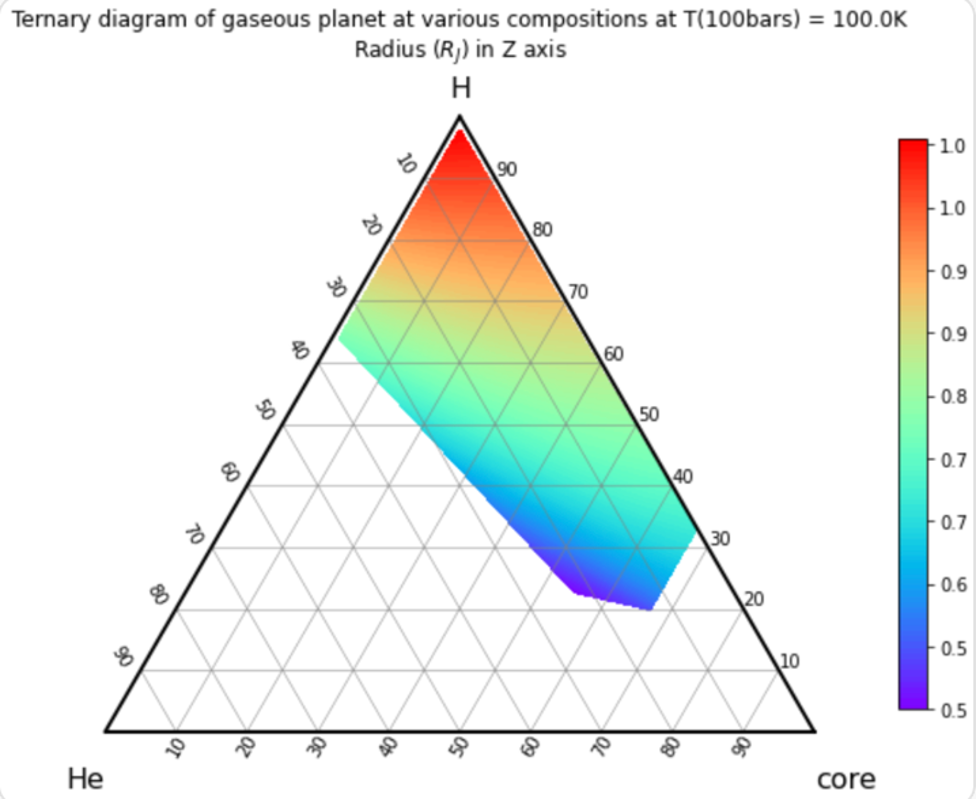
\includegraphics[width=0.48\textwidth]{Images/degeneracies.png}
    \caption{Degeneracy plot (ternary plot), representing radius ($R_J$) at various, hydrogen, helium and core mass fractions}
    \label{fig:Degen}
\end{figure}

\section{Notes on exorem model selection}

As stated in the model description, exorem can in certain conditions struggle to converge. This happens generally in zones of the grid where the irradiation temperature is low and internal temperature high. Exorem can not balance the two stream flux model and balance the temperature at the bottom and top of the atmosphere. To deal with this, we help Exorem converge either by relying on T. Guillot (2010) \parencite{guillot_radiative_2010} non grey analytical model to provide initial pressure temperature profiles to guide exorem, these do not take into account irradiation. We can also re-inject profiles from the grid into Exorem, to accomplish this we find the closest profile to the given input parameters. However often this does not suffice and we still have non-converged profiles. It would be taking a risk to leave these profiles in the grid especially taking into account that for the moment we do not use any smoothing in the interpolation methods considered above. As such we chose to remove these profiles. Through trial and error it was shown that a systematic code to identify bad profiles was inefficient. As such a simple tree based model was used to identify such profiles. To do this a LGBM classifier was trained. LGBM classifiers are gradient boosted tree based learning algorithms that have low memory usage and are more efficient than most other classifiers such as random forests. They use leaf wise tree growth which increases efficiency. The disadvantage of such classifiers are that they are very sensitive to over-fitting and require relatively large data-sets. The model was trained using the top atmosphere flux ratio, bottom atmosphere flux ratio, effective temperature ratio, internal temperature and irradiation temperature. The more data science orientated reader might be concerned when seeing that dimensional data was used as a feature. We allowed ourselves to do this as the internal temperature and irradiation temperature are bounded by the grid limits, rigorously one should divide these values by their maximum value on the grid. The results obtained were an accurate categorisation of 98\% of profiles, with an equal split percentage wise between false positives and false negatives. 

\section{Notes on entropy of mixes}

As shown in \parencite{chabrier_new_2019}, the expression for a given extensive quantity $W$ at a given $(T,P)$ for a mixture is given by :

\begin{align} 
    W(T,P) = \sum_{i} X_{i} W_{i}(T,P)
    \label{eq:extensive_qty}
\end{align}

With :

\begin{align} 
    X_{i} = \frac{M_i}{\sum_{i}M_{i}}
    \label{eq:mass_fraction}
\end{align}

Subsequently we can express the entropy of a mix of $He/H/H_2O$ as follows :

\begin{align} 
    S = \sum_{i} X_{i} S_{i}(T,P) + S_{mix}(T,P)
    \label{eq:entropy_mix1}
\end{align}

\begin{align} 
    S = X_{H} S_{H}(T,P) + X_{He} S_{He}(T,P) \nonumber \\ 
    + X_{H_2O} S_{H_2O}(T,P) + S_{mix}(T,P)
    \label{eq:entropy_mix2}
\end{align}

With here $S_{mix}(T,P)$ the ideal mixing term that we will better define subsequently. But we shall consider equal to zero.

We need to substitute the expressions for the mass fractions.  ' to remove this section.
%------------------------------------

\section{Notes on interpolation}

In a 2d space interpolations car be relatively simple, let's consider the following :

\begin{align} 
    (x,y) \in (R,R)
\end{align}

Let us suppose there is some kind of function linking the two, we hence have :

\begin{align} 
    f(x) = y
\end{align}

Should we consider two points of the function $(x_0,y_0)$ and $(x_1,y_1)$ and seek to find the value of a given unknown third point $(x_a,y_a)$ then one would instinctively do a linear interpolation as follows :

\begin{align} 
    \frac{x_1-x_0}{y_1-y_0} (x_a-x_0) + y_0 = y_a
    \label{eq:interp1d}
\end{align}

Should we desire to interpolate at a higher order, we can use the Lagrange set of polynomes as follows:

\begin{align} 
    y(x) = \sum_{j=0}^{k} y_j c_j(x)
        c_j(x) = \ell_j(x,x_0,x_1,\ldots,x_k) = \nonumber \\
        \prod_{\begin{smallmatrix}0\le m\le k\\ m\neq j\end{smallmatrix}} \frac{x-x_m}{x_j-x_m} = \nonumber \\
        \frac{(x-x_0)}{(x_j-x_0)} \cdots \frac{(x-x_{j-1})}{(x_j-x_{j-1})} \frac{(x-x_{j+1})}{(x_j-x_{j+1})} \cdots \frac{(x-x_k)}{(x_j-x_k)}
\end{align}

For a polynome of order $k$ we require $k+1$ node points, this is an important point to keep in mind when constructing a grid to subsequently interpolate. Interpolation residuals will not be detailed here. As all that is explicated here can be found in any math book, the more curious reader can quite easily find further details.

Another way of of seeing \cref{eq:interp1d} is as evaluating the barycenter along a line. where the term $x_a-x_0$ represents the displacement from $x_0$ to $x$. Generalised, it is possible to write the higher order polynomial approximation in terms of the displacement from a given point.

\begin{align} 
    L(x) = \ell(x) \sum_{j=0}^k \frac{w_j}{x-x_j}y_j
\end{align}

In practice this means that we consider a set of values $f(x_j)=y_j$ close to the desired point and interpolate the point by weighting the $f(x_j)$ values by the distance $x-x_j$ to that given point.

That which is given here is valid in a two dimensional space but for parts of the work, it is required to interpolate in higher dimension. To quote "Méthode numériques appliquées" by Jean-Philippe Grivet \parencite{Methodes_numerique_appliques} : "The algorithms described above can be generalized in a more or less laborious way to two or more dimensions." This has been one of the challenges to overcome in this work. Indeed for perfectly regular grids, it is possible to derive semi-analytical equations using methods such as bi-cubic interpolations, however here our grids will, through iterative steps, no longer be regular. We propose to overcome this problem to use a barycentric interpolation using a Delauney triangulation. In terms of the barycentric interpolation the method is the same as the logic presented above. We weight the distance between nodes by the distance to the desired point and that for a group of points that surround our point of interest. However the surrounding of a point in higher dimension is a non negligible task. A Delaunay triangulation in a two dimensional space is a triangulation for which no point of the grid is in the circumcircle of another triangle, where a triangle is defined by three points of the grid. If one draws this condition out one will notice that this splits a space into triangles with no points inside those triangles. For a higher dimensional space, the circumcircle becomes a circum-hypersphere. The mathematical details will be left to the most curious readers.\par

In practice, the methods presented were not coded but imported from the python Scipy library. However it is essential when using interpolations to know what is being done. Interpolations if used incorrectly can lead to erroneous results which can appear correct. For this reason we do not explicit extrapolations as any desired data points outside of the grid are deemed only accessible if the grid is extended by running the underlying models. This poses a new challenge, how to correctly extend the grid in order to subsequently perform interpolations. If computational time is plenteous than a random grid search can be completed, otherwise an extrapolation can be carried out with the objective of running the underlying models at the extrapolation point. This is yet to be correctly done.

\section{Notes on degeneracy}

\Cref{fig:Degen} gives an example of partial ternary degeneracy plot generated with Exoris where we see how the radius for a planet at a given mass varies depending on its mass fraction composition. Where the color is the same, we have a degeneracy. We see that it is possible to have the same radius for various mass fractions of hydrogen, helium and core. This plot explicates the need to link interior models with atmosphere models. Indeed the hydrogen and helium mass fractions here are ultimately fixed by the atmosphere model. The core is therefore left as a free parameter, however if the radius of a planet is known it is possible to remove all degeneracy presented here. The more critical reader could think that fundamentally this is just pushing the problem up into the atmosphere, this is true, however as photons escape from radiative zones in the atmosphere, it is theoretically possible with a perfect observation to resolve this internal structure as presented here. However internal structures can be more complex than this diagram indicates. The core can have rock and ice composition, with distinct fractions of both. We can also imagine for Neptune like planets layers of water/ice in the envelope, in which case the degeneracy plot becomes more complicated and further work is required in order to understand what remains degenerate after model linkage.

\begin{figure}
    \centering
    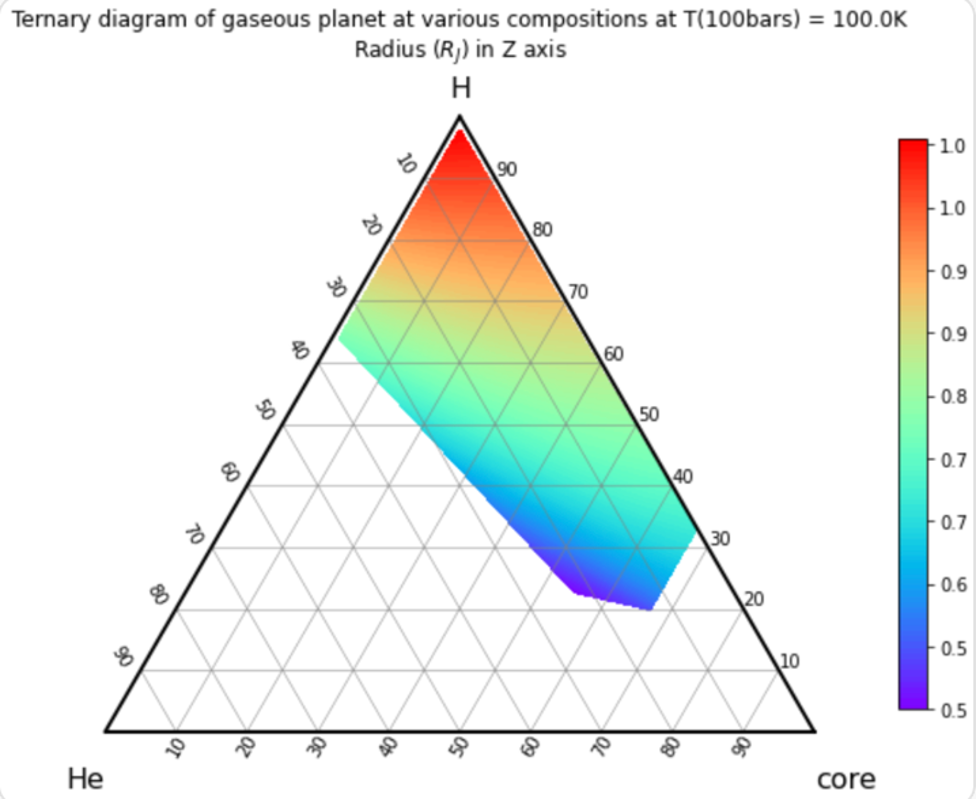
\includegraphics[width=0.48\textwidth]{Images/degeneracies.png}
    \caption{Degeneracy plot (ternary plot), representing radius ($R_J$) at various, hydrogen, helium and core mass fractions}
    \label{fig:Degen}
\end{figure}

\section{Notes on exorem model selection}

As stated in the model description, exorem can in certain conditions struggle to converge. This happens generally in zones of the grid where the irradiation temperature is low and internal temperature high. Exorem can not balance the two stream flux model and balance the temperature at the bottom and top of the atmosphere. To deal with this, we help Exorem converge either by relying on T. Guillot (2010) \parencite{guillot_radiative_2010} non grey analytical model to provide initial pressure temperature profiles to guide exorem, these do not take into account irradiation. We can also re-inject profiles from the grid into Exorem, to accomplish this we find the closest profile to the given input parameters. However often this does not suffice and we still have non-converged profiles. It would be taking a risk to leave these profiles in the grid especially taking into account that for the moment we do not use any smoothing in the interpolation methods considered above. As such we chose to remove these profiles. Through trial and error it was shown that a systematic code to identify bad profiles was inefficient. As such a simple tree based model was used to identify such profiles. To do this a LGBM classifier was trained. LGBM classifiers are gradient boosted tree based learning algorithms that have low memory usage and are more efficient than most other classifiers such as random forests. They use leaf wise tree growth which increases efficiency. The disadvantage of such classifiers are that they are very sensitive to over-fitting and require relatively large data-sets. The model was trained using the top atmosphere flux ratio, bottom atmosphere flux ratio, effective temperature ratio, internal temperature and irradiation temperature. The more data science orientated reader might be concerned when seeing that dimensional data was used as a feature. We allowed ourselves to do this as the internal temperature and irradiation temperature are bounded by the grid limits, rigorously one should divide these values by their maximum value on the grid. The results obtained were an accurate categorisation of 98\% of profiles, with an equal split percentage wise between false positives and false negatives. 

\section{Notes on entropy of mixes}

As shown in \parencite{chabrier_new_2019}, the expression for a given extensive quantity $W$ at a given $(T,P)$ for a mixture is given by :

\begin{align} 
    W(T,P) = \sum_{i} X_{i} W_{i}(T,P)
    \label{eq:extensive_qty}
\end{align}

With :

\begin{align} 
    X_{i} = \frac{M_i}{\sum_{i}M_{i}}
    \label{eq:mass_fraction}
\end{align}

Subsequently we can express the entropy of a mix of $He/H/H_2O$ as follows :

\begin{align} 
    S = \sum_{i} X_{i} S_{i}(T,P) + S_{mix}(T,P)
    \label{eq:entropy_mix1}
\end{align}

\begin{align} 
    S = X_{H} S_{H}(T,P) + X_{He} S_{He}(T,P) \nonumber \\ 
    + X_{H_2O} S_{H_2O}(T,P) + S_{mix}(T,P)
    \label{eq:entropy_mix2}
\end{align}

With here $S_{mix}(T,P)$ the ideal mixing term that we will better define subsequently. But we shall consider equal to zero.

We need to substitute the expressions for the mass fractions.  ' to remove this section.
%------------------------------------

\section{Notes on interpolation}

In a 2d space interpolations car be relatively simple, let's consider the following :

\begin{align} 
    (x,y) \in (R,R)
\end{align}

Let us suppose there is some kind of function linking the two, we hence have :

\begin{align} 
    f(x) = y
\end{align}

Should we consider two points of the function $(x_0,y_0)$ and $(x_1,y_1)$ and seek to find the value of a given unknown third point $(x_a,y_a)$ then one would instinctively do a linear interpolation as follows :

\begin{align} 
    \frac{x_1-x_0}{y_1-y_0} (x_a-x_0) + y_0 = y_a
    \label{eq:interp1d}
\end{align}

Should we desire to interpolate at a higher order, we can use the Lagrange set of polynomes as follows:

\begin{align} 
    y(x) = \sum_{j=0}^{k} y_j c_j(x)
        c_j(x) = \ell_j(x,x_0,x_1,\ldots,x_k) = \nonumber \\
        \prod_{\begin{smallmatrix}0\le m\le k\\ m\neq j\end{smallmatrix}} \frac{x-x_m}{x_j-x_m} = \nonumber \\
        \frac{(x-x_0)}{(x_j-x_0)} \cdots \frac{(x-x_{j-1})}{(x_j-x_{j-1})} \frac{(x-x_{j+1})}{(x_j-x_{j+1})} \cdots \frac{(x-x_k)}{(x_j-x_k)}
\end{align}

For a polynome of order $k$ we require $k+1$ node points, this is an important point to keep in mind when constructing a grid to subsequently interpolate. Interpolation residuals will not be detailed here. As all that is explicated here can be found in any math book, the more curious reader can quite easily find further details.

Another way of of seeing \cref{eq:interp1d} is as evaluating the barycenter along a line. where the term $x_a-x_0$ represents the displacement from $x_0$ to $x$. Generalised, it is possible to write the higher order polynomial approximation in terms of the displacement from a given point.

\begin{align} 
    L(x) = \ell(x) \sum_{j=0}^k \frac{w_j}{x-x_j}y_j
\end{align}

In practice this means that we consider a set of values $f(x_j)=y_j$ close to the desired point and interpolate the point by weighting the $f(x_j)$ values by the distance $x-x_j$ to that given point.

That which is given here is valid in a two dimensional space but for parts of the work, it is required to interpolate in higher dimension. To quote "Méthode numériques appliquées" by Jean-Philippe Grivet \parencite{Methodes_numerique_appliques} : "The algorithms described above can be generalized in a more or less laborious way to two or more dimensions." This has been one of the challenges to overcome in this work. Indeed for perfectly regular grids, it is possible to derive semi-analytical equations using methods such as bi-cubic interpolations, however here our grids will, through iterative steps, no longer be regular. We propose to overcome this problem to use a barycentric interpolation using a Delauney triangulation. In terms of the barycentric interpolation the method is the same as the logic presented above. We weight the distance between nodes by the distance to the desired point and that for a group of points that surround our point of interest. However the surrounding of a point in higher dimension is a non negligible task. A Delaunay triangulation in a two dimensional space is a triangulation for which no point of the grid is in the circumcircle of another triangle, where a triangle is defined by three points of the grid. If one draws this condition out one will notice that this splits a space into triangles with no points inside those triangles. For a higher dimensional space, the circumcircle becomes a circum-hypersphere. The mathematical details will be left to the most curious readers.\par

In practice, the methods presented were not coded but imported from the python Scipy library. However it is essential when using interpolations to know what is being done. Interpolations if used incorrectly can lead to erroneous results which can appear correct. For this reason we do not explicit extrapolations as any desired data points outside of the grid are deemed only accessible if the grid is extended by running the underlying models. This poses a new challenge, how to correctly extend the grid in order to subsequently perform interpolations. If computational time is plenteous than a random grid search can be completed, otherwise an extrapolation can be carried out with the objective of running the underlying models at the extrapolation point. This is yet to be correctly done.

\section{Notes on degeneracy}

\Cref{fig:Degen} gives an example of partial ternary degeneracy plot generated with Exoris where we see how the radius for a planet at a given mass varies depending on its mass fraction composition. Where the color is the same, we have a degeneracy. We see that it is possible to have the same radius for various mass fractions of hydrogen, helium and core. This plot explicates the need to link interior models with atmosphere models. Indeed the hydrogen and helium mass fractions here are ultimately fixed by the atmosphere model. The core is therefore left as a free parameter, however if the radius of a planet is known it is possible to remove all degeneracy presented here. The more critical reader could think that fundamentally this is just pushing the problem up into the atmosphere, this is true, however as photons escape from radiative zones in the atmosphere, it is theoretically possible with a perfect observation to resolve this internal structure as presented here. However internal structures can be more complex than this diagram indicates. The core can have rock and ice composition, with distinct fractions of both. We can also imagine for Neptune like planets layers of water/ice in the envelope, in which case the degeneracy plot becomes more complicated and further work is required in order to understand what remains degenerate after model linkage.

\begin{figure}
    \centering
    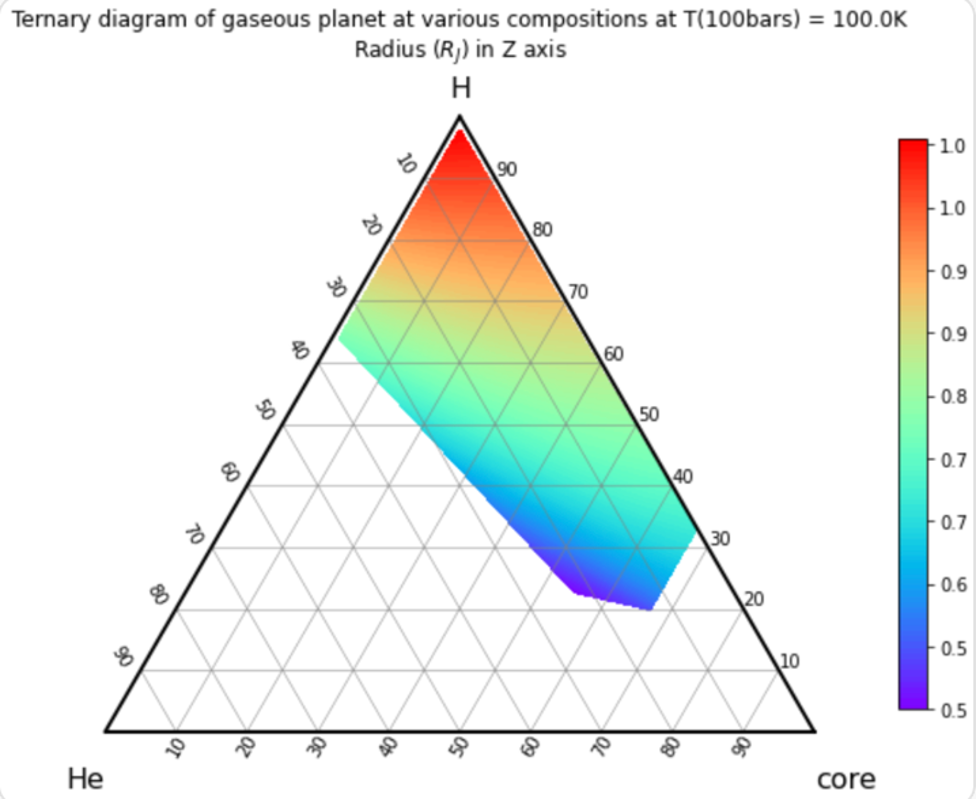
\includegraphics[width=0.48\textwidth]{Images/degeneracies.png}
    \caption{Degeneracy plot (ternary plot), representing radius ($R_J$) at various, hydrogen, helium and core mass fractions}
    \label{fig:Degen}
\end{figure}

\section{Notes on exorem model selection}

As stated in the model description, exorem can in certain conditions struggle to converge. This happens generally in zones of the grid where the irradiation temperature is low and internal temperature high. Exorem can not balance the two stream flux model and balance the temperature at the bottom and top of the atmosphere. To deal with this, we help Exorem converge either by relying on T. Guillot (2010) \parencite{guillot_radiative_2010} non grey analytical model to provide initial pressure temperature profiles to guide exorem, these do not take into account irradiation. We can also re-inject profiles from the grid into Exorem, to accomplish this we find the closest profile to the given input parameters. However often this does not suffice and we still have non-converged profiles. It would be taking a risk to leave these profiles in the grid especially taking into account that for the moment we do not use any smoothing in the interpolation methods considered above. As such we chose to remove these profiles. Through trial and error it was shown that a systematic code to identify bad profiles was inefficient. As such a simple tree based model was used to identify such profiles. To do this a LGBM classifier was trained. LGBM classifiers are gradient boosted tree based learning algorithms that have low memory usage and are more efficient than most other classifiers such as random forests. They use leaf wise tree growth which increases efficiency. The disadvantage of such classifiers are that they are very sensitive to over-fitting and require relatively large data-sets. The model was trained using the top atmosphere flux ratio, bottom atmosphere flux ratio, effective temperature ratio, internal temperature and irradiation temperature. The more data science orientated reader might be concerned when seeing that dimensional data was used as a feature. We allowed ourselves to do this as the internal temperature and irradiation temperature are bounded by the grid limits, rigorously one should divide these values by their maximum value on the grid. The results obtained were an accurate categorisation of 98\% of profiles, with an equal split percentage wise between false positives and false negatives. 

\section{Notes on entropy of mixes}

As shown in \parencite{chabrier_new_2019}, the expression for a given extensive quantity $W$ at a given $(T,P)$ for a mixture is given by :

\begin{align} 
    W(T,P) = \sum_{i} X_{i} W_{i}(T,P)
    \label{eq:extensive_qty}
\end{align}

With :

\begin{align} 
    X_{i} = \frac{M_i}{\sum_{i}M_{i}}
    \label{eq:mass_fraction}
\end{align}

Subsequently we can express the entropy of a mix of $He/H/H_2O$ as follows :

\begin{align} 
    S = \sum_{i} X_{i} S_{i}(T,P) + S_{mix}(T,P)
    \label{eq:entropy_mix1}
\end{align}

\begin{align} 
    S = X_{H} S_{H}(T,P) + X_{He} S_{He}(T,P) \nonumber \\ 
    + X_{H_2O} S_{H_2O}(T,P) + S_{mix}(T,P)
    \label{eq:entropy_mix2}
\end{align}

With here $S_{mix}(T,P)$ the ideal mixing term that we will better define subsequently. But we shall consider equal to zero.

We need to substitute the expressions for the mass fractions. 